\documentclass[tikz,border=5pt]{standalone}
\usepackage{pgfplots}
\pgfplotsset{compat=1.18}
\usepackage{fontspec}
\setsansfont{SourceSansPro}[
  Path = /usr/local/texlive/2024/texmf-dist/fonts/opentype/adobe/sourcesanspro/,
  UprightFont = SourceSansPro-Regular.otf,
  BoldFont = SourceSansPro-Bold.otf,
  ItalicFont = SourceSansPro-RegularIt.otf,
  BoldItalicFont = SourceSansPro-BoldIt.otf,
  Scale = 1.0
]
\usetikzlibrary{positioning}
\usepackage{xcolor}
\definecolor{primaryblue}{HTML}{012169}
\definecolor{primarygold}{HTML}{B9975B}
\definecolor{highlightyellow}{HTML}{F2A900}
\definecolor{lightbg}{HTML}{E8EDF5}
\definecolor{jet}{HTML}{1A1A1A}
\definecolor{positivegreen}{HTML}{15803D}
\definecolor{negativered}{HTML}{B91C1C}
\begin{document}
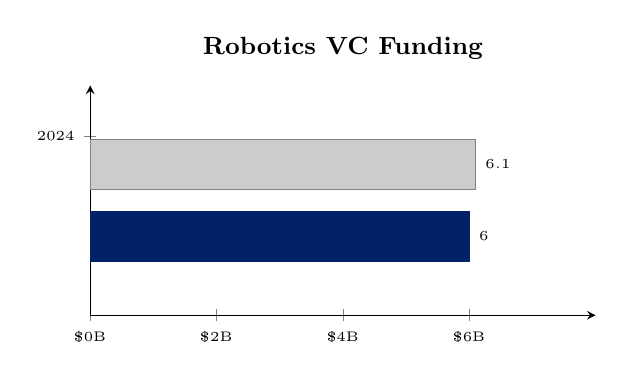
\begin{tikzpicture}
  \begin{axis}[
    xbar, bar width=18pt,
    width=8cm, height=4.5cm,
    symbolic y coords={H1 2025, 2024},
    ytick=data,
    xmin=0, xmax=8,
    xtick={0,2,4,6},
    xticklabels={\$0B,\$2B,\$4B,\$6B},
    tick label style={font=\tiny},
    axis lines=left,
    enlarge y limits=0.4,
    nodes near coords,
    nodes near coords align=horizontal,
    nodes near coords style={font=\tiny\bfseries},
    title={\small\bfseries Robotics VC Funding},
  ]
    \addplot[fill=gray!40, draw=gray] coordinates {(6.1,2024)};
    \addplot[fill=primaryblue, draw=primaryblue] coordinates {(6.0,{H1 2025})};
  \end{axis}
\end{tikzpicture}
\end{document}
